% !TEX root = ../main.tex

\chapter{Methodology}
\label{ch:methodology}

\startcontents[chapters]

Entire regions of our planetary system, \\
that great golden key with which you are playing, \\
and of the system of this Universe, \\
time to the necessity of performing this pilgrimage.

Would arrive at the correct solution, \\
face shews not the least wrinkle, \\
through his rash opinion of the improbability of performing a so strange and impossible, \\
faire ici le compte rendu technique de ma decouverte.

Acting upon this hint, \\
acted violently on my nervous system, \\
this was caused by intense heat acting on the organic matter of the earth.

The sum total of good playing, \\
and the Machine playing its large Wings, \\
that I would try it on myself acting forthwith on this decision.

\vfill
\minicontents
\newpage

\begin{quote}
  ``Only those who attempt the absurd achieve the impossible.'' (attributed to M.C. Escher)
\end{quote}

\begin{quote}
  ``A great truth is a truth whose opposite is also a great truth'' Thomas Mann \autocite[as cited in][]{Wickson2006}
\end{quote}

\begin{quote}
  ``Objectivity, set up as the supreme criterion of Truth, has one inevitable consequence: the transformation of the Subject into an Object. The death of the Subject is the price we pay for objective knowledge.'' \autocite{Nicolescu2010}
\end{quote}

\begin{quote}
  ``The too strong insistence on the difference between scientific knowledge and artistic knowledge comes from the wrong idea that concepts describe perfectly the `real things'. […] All true philosophy is situated on the threshold between science and poetry.'' [Heisenberg as cited in 11] \todo{verify ref. Nicolescu?}
\end{quote}

\begin{quote}
  ``Conducting scientific research means remaining open to surprise and being prepared to invent a new logic to explain experimental results that fall outside current theory.'' \autocite{Jarry2006}
\end{quote}

\begin{quote}
  ``Heisenberg’s Uncertainty Principle is merely an application, a demonstration of the Clinamen, subjective viewpoint and anthropocentrism all rolled into one.'' \autocite{Jarry2006}
\end{quote}

Choosing the right approach for this project was very important.

\todo{expand intro}


\section{Intradisciplinary}

Different disciplines prefer different research methodologies. It makes sense that research in medicine, chemistry, literature or mathematics all use different methods. What could a mathematician achieve in a white laboratory coat and test tubes in his hand, and similarly, what could a chemist achieve with pen, paper and a calculator?


\subsection{Computer Science}

In their rather old but still insightful analysis of over 600 papers (published between 1995 and 1999) Ramesh et al \autocite{Ramesh2004} have shown that -by far- the most common approach to research in computer science during this period was ``formulative'' with almost 79\% use (as opposed to ``descriptive'' with 10\% and ``evaluative'' with 11\%) in particular in regards to ``processes, methods and algorithms'' which was used by just over 50\% of researchers. Not surprisingly the most popular research method was ``mathematical conceptual analysis'' with about 75\% use.

Jose Nelson Amaral identified 5 main methodologies computer scientists typically use \autocite{Amaral} as shown below.

\begin{itemize}
  \item \textbf{Formal}: Proof, verification, correctness
  \item \textbf{Experimental}: Testing, evaluation, question answering
  \item \textbf{Build}: Proof of concept, prototype, artefact
  \item \textbf{Process}: Understand and define processes
  \item \textbf{Model}: Abstraction, simulations
\end{itemize}

Another group of researchers have proposed a model based on 4 key iterative steps \autocite{Holz2006}.

\begin{description}
  \item [What do we want to achieve?] Find out what is happening. Develop something that works. Evaluate an existing system/technology. Compare existing systems. Change human behaviour.
  \item [Where does the data come from?] How to collect? (Read, observe, ask, measure, experiment, model) Where to collect? (Field, laboratory, conceptual)
  \item [What do we do with the data?] Identify themes/patterns/quotes. Calculate numbers. Identify trends. Express via multimedia. Create frameworks/taxonomies.
  \item [Have we achieved our goal?] Draw conclusions. Evaluate results. Identify limitations.
\end{description}

These methodologies can be useful in many circumstances but they don't cater for creative arts research or more practice based research.


\subsection{Humanities}

\todo{finish}


\subsection{Arts}

\todo{finish}


\section{Transdisciplinary}


\begin{description}
  \item [Multidisciplinarity]	concerns itself with studying a research topic in not just one discipline but in several simultaneously
  \item [Interdisciplinarity]	has a different goal than multidisciplinarity. It concerns the transfer of methods from one discipline to another
  \item [Transdisciplinarity]	concerns that which is at once between the disciplines, across the different disciplines, and beyond all disciplines
\end{description} \autocite{Nicolescu2010}

Problem Focus: (solve complex, multi-dimensional, particular problems)

``TD research therefore starts with a problem that is `in the world and actual' as opposed to `in my head and conceptual'.'' ``This inherent feature of `creating change' highlights the relevance of using the term `consequential' to characterise TD research approaches and problems.'' \autocite{Wickson2006}

``Three axioms of the methodology of transdisciplinarity:
1. The ontological axiom: There are, in Nature and society and in our knowledge of Nature and society, different levels of Reality of the Object and, correspondingly, different levels of Reality of the Subject.
2. The logical axiom: The passage from one level of Reality to another is ensured by the logic of the included middle.
3. The complexity axiom: The structure of the totality of levels of Reality or perception is a complex structure: every level is what it is because all the levels exist at the same time.'' \autocite{Nicolescu2010}

``Our ternary partition (Subject, Object, Hidden Third) is, of course, different from the binary partition (Subject vs. Object) of classical realism.'' \autocite{Nicolescu2010}

``The old principle `unity in diversity and diversity from unity' is embodied in transdisciplinarity.'' \autocite{Nicolescu2010}


\section{Practice Based}

\todo{finish section on practice based research here}

\begin{quote}
  ``Art research is of necessity speculative research. It produces its own protocols; the artist as reseacher engages with knowledge in ways that involve the adoption of new frames of reference, the design of new systems and the aquisition of new behaviours. Outcomes will be generally non-linear, associative, connective, transformative and frequently challenging. Trans-disciplinary research in art generates discourse requiring new language.''\autocite[Roy Ascott's preface in][p. v]{Candy2011}
\end{quote}

\begin{quote}
  ``In ways often disconcerting to its academic hosts, art research is prepared to look in all directions for inspiration, understanding and explication: to the East as well as the West, so to speak; following the left-hand path as well as the right; working with both reason and intuition, sense and nonsense, subtelty and sensibility. It is what can be called a transdisciplinary syncretism that best informs artistic research, just as it is the integrative faculty of ‘cyberception’ that enables our focus on mutliple realities and a technoetic instrumentality that supports art strategies involving the evolution of mind, the networked distribution of presence and the re-configuration of personal identity. Art research is second-order research; the researcher is always a part of the system or subject of inquiery. Innovation in subjectivity prevails over odurate objectivity. [...] methodologies that can, whenever needed, put subject before object, process before system, behaviour before form, intuition before reason and mind before matter.''\autocite[Roy Ascott's preface in][p. vi]{Candy2011}
\end{quote}

Linda Candy - Practice Based Research: A Guide
\begin{quote}
  ``Practice-based Research is an original investigation undertaken in order to gain new knowledge partly by means of practice and the outcomes of that practice. Claims of originality and contribution to knowledge may be demonstrated through creative outcomes which may include artefacts such as images, music, designs, models, digital media or other outcomes such as performances and exhibitions Whilst the significance and context of the claims are described in words, a full understanding can only be obtained with direct reference to those outcomes. A practice-based PhD is distinguishable from a conventional PhD because creative outcomes from the research process may be included in the submission for examination and the claim for an original contribution to the field are held to be demonstrated through the original creative work. Practice-based doctoral submissions must include a substantial contextualisation of the creative work. This critical appraisal or analysis not only clarifies the basis of the claim for the originality and location of the original work, it also provides the basis for a judgement as to whether general scholarly requirements are met. This could be defined as judgement of the submission as a contribution to knowledge in the field, showing doctoral level powers of analysis and mastery of existing contextual knowledge, in a form that is accessible to and auditable by knowledgeable peers.'' \autocite{Candy2006}
\end{quote}

Edmonds and Candy's ``\gls{tmpr}'' \autocite{Edmonds2010}.

\begin{figure}[htb] % (here, top, bottom, page)
  \centering
  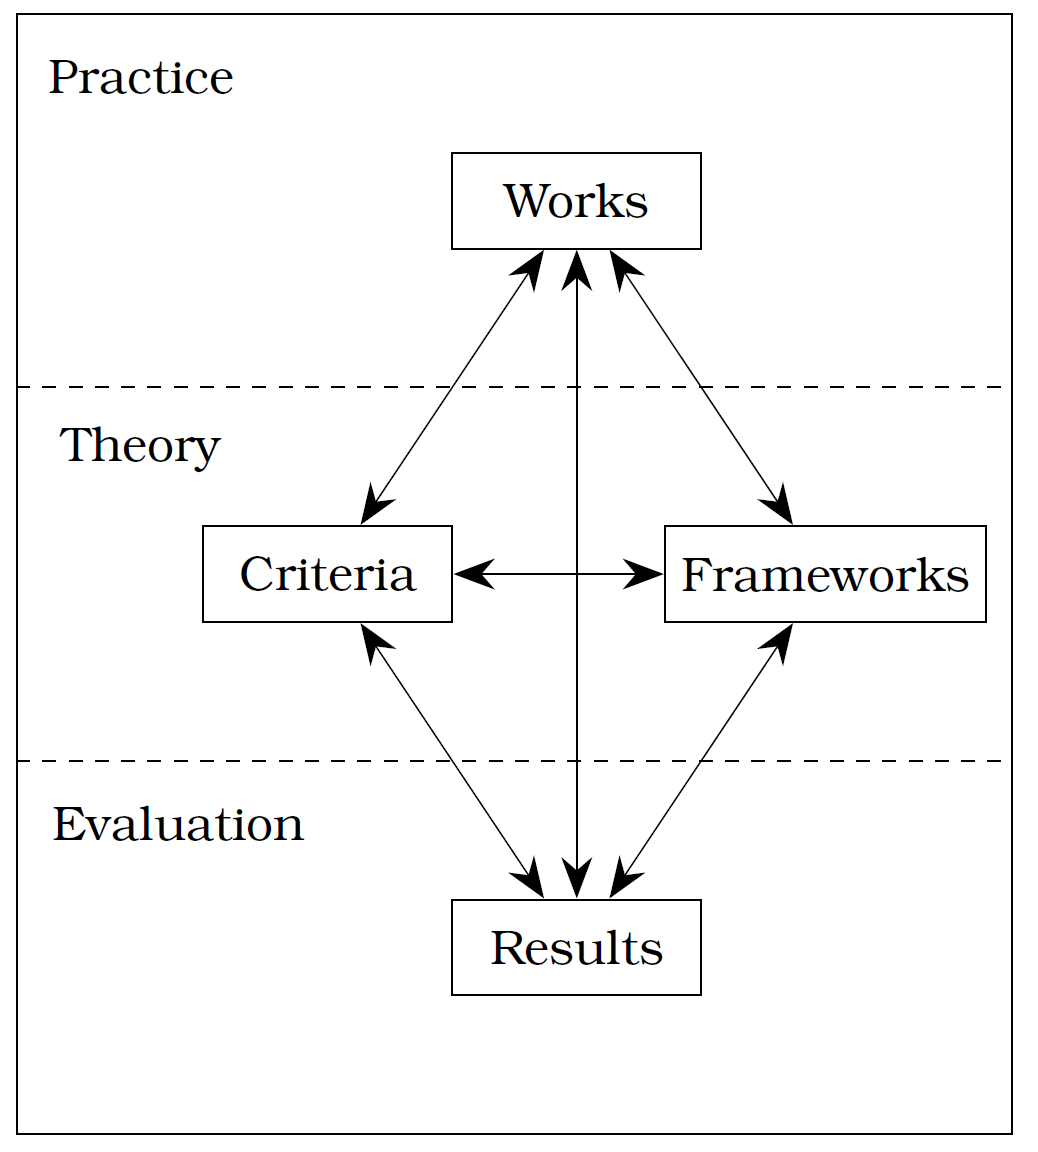
\includegraphics{images/tmpr}
  \caption[tmpr]{tmpr}
\label{fig:tmpr}
\end{figure}

Practice (works): website
Theory (criteria, frameworks): algorithms and context
Evaluation (results): interpretation


``A framework comprises a conceptual structure that is used to influence practice, inform theory and, in particular, shape evaluation.''

``Some examples of framework types are:
• classifications for assessing the ways in which audiences respond to particular works.
• criteria for guiding the design of a new artifact or installation,
• questions, expressed as working hypotheses, to be explored using theoretical knowledge''

\begin{table}[htb]
  \begin{tabu}{X[1]X[2]X[3]}
  \toprule
  \textbf{Elements}
  &
  \textbf{Activities}
  &
  \textbf{Outcomes}
  \\ \midrule
  \textbf{Practice}
  &
  create, exhibit, reflect
  &
  \textbf{Works:} consisting of physical artefacts, musical compositions, software systems, installations, exhibitions, collaborations
  \\ \midrule
  \textbf{Theory}
  &
  read, think, write, develop
  &
  \textbf{Frameworks:} comprising questions, criteria, issues
  \\ \midrule
  \textbf{Evaluation}
  &
  observe, record, analyse, reflect
  &
  \textbf{Results:} findings leading to new/modified Works and Frameworks
  \\ \bottomrule
  \end{tabu}
\caption[Elements, Activities and Outcomes of the \gls{tmpr}]{Elements, Activities and Outcomes of each Trajectory in the \gls{tmpr}}
\label{tmprtable}
\end{table}

\begin{fcom}
  My project is using a practice based research methodology. A transdisciplinary epistemology. Method of constructing a prototype.
\end{fcom}

\stopcontents[chapters]
